
\documentclass[lnicst]{svmultln}
\renewcommand{\arraystretch}{1.5}
\usepackage{amssymb}
\setcounter{tocdepth}{3}

\usepackage{epsfig}
\usepackage{cite}
\usepackage{verbatim}
\usepackage{graphicx}
\usepackage{caption}
\usepackage{subcaption}

\usepackage{url}
\urldef{\mailsa}\path|{collins, rajive}@cs.ucla.edu|
\usepackage[pdfpagelabels,hypertexnames=false,breaklinks=true,bookmarksopen=true,bookmarksopenlevel=2]{hyperref}

\begin{document}

\mainmatter  % start of an individual contribution

% first the title is needed
\title{MELON: A Persistent Message-Based Communication Paradigm for MANETs}

\titlerunning{MELON Communication Paradigm for MANETs}

\author{Justin Collins\and Rajive Bagrodia}
\authorrunning{MELON Communication Paradigm for MANETs}
% (feature abused for this document to repeat the title also on left hand pages)

% the affiliations are given next
\institute{University of California, Los Angeles\\
Los Angeles, CA\\
\mailsa }

\toctitle{MELON: A Persistent Message-Based Communication Paradigm for MANETs}
\tocauthor{Justin Collins and Rajive Bagrodia}


\maketitle
\begin{abstract}
In this paper we introduce MELON, a new communication paradigm tailored to mobile ad hoc networks, based on novel interactions with a distributed shared message store. MELON provides remove-only, read-only, and private messages, as well as bulk message operations. The dynamic nature of MANETs is addressed with persistent messages, completely distributed message storage, and flexible communication patterns. We quantitatively compare a prototype implementation of MELON to existing paradigms to show its feasibility as the basis for new MANET applications. Experiments demonstrate 40\% better throughput on average than traditional paradigms, as well as 70\% faster local insertion and removal operations compared to an existing tuple space library.
\end{abstract}

\section{Introduction}

While smartphones are quickly becoming ubiquitous, most mobile applications continue to use a client-server model rather than communicating through mobile ad hoc networks (MANET). One reason may be the added challenges of developing a MANET application which must communicate with peers over unreliable shifting network topologies. While communicating over a single-hop wireless network (e.g., a WiFi access point or cellular tower) to a central server is simpler, MANETs are useful when communication is between nearby devices or when there is no network infrastructure, such as in disaster recovery situations or locations without cellular service.

To alleviate application development challenges posed by MANETs, several approaches to middleware and libraries have been proposed. The majority of these proposals are adapted forms of traditional distributed computing paradigms such as publish/subscribe, remote procedure calls, and tuple spaces, instead of MANET-focused paradigms\cite{mine}.

In this paper, we introduce a new paradigm called MELON\footnote{Message Exchange Language Over the Network}. MELON overcomes frequent network disconnections in MANETs by providing message persistence in a distributed shared message store and can operate entirely on-demand, avoiding coupling between nodes. MELONs offer remove-only, read-only, and private messages, as well as bulk transfers. MELON also simplifies communication by returning messages in per host write order. We demonstrate that our proposed paradigm is practical by comparing performance of a prototype MELON implementation to canonical implementations of traditional paradigms in a MANET environment. Results show higher throughput with comparable latency.

%The rest of this paper is organized as follows: Section \ref{sec:challenges} lists the MANET challenges we address; Section \ref{sec:design} discusses the design and operations of MELON; Section \ref{sec:implementation} provides details of the MELON implementation; in Section \ref{sec:evaluation} we quantitatively compare MELON to existing paradigms; Section \ref{sec:relatedwork} references related work; and finally Section \ref{sec:conclusion} presents our conclusions.

%\section{MANET Application Challenges}\label{sec:challenges}


%Wireless communication can be disrupted in many ways, including competing broadcasts, physical obstacles, and nodal mobility. When combined with an entirely self-organizing network where nodes may join and leave the network at any time, this environment leads to frequent communication disruptions. In traditional networking libraries, disconnections are treated as exceptional events which must be handled by the application. In MANETs, disconnections are so common they should be handled naturally by the programming paradigm.

%The dynamicity of MANETs also leads to transience of resources. It is common in distributed programming paradigms to refer to resources independently from the physical location of the resources. This also works well in MANETs, since a resource is likely to be mobile, and several hosts may offer the same type of resource over time.

%Before addressing resources an application must discover the resources which are available. The infrastructureless nature of MANETs precludes the use of centralized architectures to maintain a directory of resources. It is also unlikely the location of resources will be known prior to joining a network. Distributed discovery mechanisms are needed to find resources in a MANET environment.

%As the primary purpose of a programming paradigm for MANETs is communication between hosts, a general-purpose paradigm should provide flexible communication: both multicast and unicast communication are common in MANET applications. Given the ubiquity of SMS, instant messaging, and direct messages, the paradigm should also support private unicast communication.

%It should also be noted that devices in MANETs are often resource constrained. Smartphones have become essentially ubiquitous in many locales but have much less power, CPU, memory, and storage space than a typical desktop computer. These constraints influence the design of paradigms intended for these devices.

\section{MELON Design}\label{sec:design}

Applications which are developed for MANETs must operate in an infrastructureless, unreliable, and dynamic distributed environment. We consider disconnection handling, addressing and discovery, and flexible communication important features for MANET development.

The design of MELON is built around a distributed shared message store. Each device in the network may host any number of applications which access and contribute to the shared message store. Each application hosts a local message store which may be accessed by any local or remote application. Applications request messages (which may be local or remote) using message templates.

By communicating through a shared message store, the concept of connections between hosts is eliminated and thus disconnections are no longer an application layer concern. Hosts suddenly leaving the network do not disrupt an application and applications do not need to handle operations failing from intermittent network connectivity or physical wireless interference. The application is insulated from these issues by the semantics of the operations.

%Messages are sent and received asynchronously by storing and retrieving them from the shared message store, removing the need for a persistent connection. This provides temporal decoupling between hosts, since messages can still be delivered even after prolonged disconnections.

%The dynamic network topology of MANETs creates a challenge which maintaining any type of logical or overlay network, so MELON does not rely on a particular network structure. Discovery of available messages is performed on-demand for each operation. While this does increase the amount of communication required for each operation, it avoids global state and allows the network to change at any time.

%MELON also provides spatial decoupling by matching messages based on content, instead of a host address or location. The messages themselves may physically reside on any host in the network. The sender of a message is not aware of the receivers' identities nor even how many receivers might read a message. This frees applications from tracking remote addresses or contacting a directory service to find remote resources.

%The shared wireless communication medium in MANETs is well-suited to multicast communications. MELON supports multicast communication by allowing any number of receivers to read the same message. MELON also provides bulk receives, which allow applications to efficiently receive multiple messages from multiple hosts in a single operation.

%Applications often also require unicast communication. While unicast communication can be accomplished by storing regular messages in MELON, these can be disrupted by a process removing a message intended for a different receiver. It is also possible to eavesdrop on messages by reading but not removing a message. For applications such as instant messaging, it is important to have private unicast communication. In MELON, messages may be directed to a specific receiver to ensure the messages are only taken by the intended recipient.

MELON also includes features uncommon to shared message stores to further simplify application development in MANETs. First, messages are returned in first-in first-out order per host. When a single host generates the majority of the messages, this removes the need to re-order messages in the application. 

Secondly, MELON provides operations to only read messages which were not previously read by the same process. This enables an application to read all matching messages currently in the message store, then read only newly-added messages in subsequent operations, avoiding the multiple read problem\cite{mrdp}.

Finally, MELON differentiates messages intended to persist and be read by many receivers from messages expected to be removed from the message store. For example, a news feed would have many readers but messages should not be removed. In contrast, in a job queue each job should be removed by exactly one worker. MELON supports both scenarios.

\subsection{MELON Operations}

\begin{table}
\scriptsize
\caption{MELON Operations}
\centering
\begin{tabular}{|c|c|c|}
\hline
\textbf{Operation} & \textbf{Return Type} & \textbf{Action} \\ \hline
\textbf{store}(\textit{message}, \textit{[address]}) & \textit{null} & Store removable message \\ \hline
\textbf{write}(\textit{message}) & \textit{null} & Store read-only message \\ \hline
\textbf{take}(\textit{template}, \textit{[block = true]}) & \textit{message} or \textit{null} & Remove and return message \\ \hline
\textbf{read}(\textit{template}, \textit{[block = true]}) & \textit{message} or \textit{null} & Copy and return read-only message \\ \hline
\textbf{take\_all}(\textit{template}, \textit{[block = true]}) & \textit{array} & Bulk remove messages \\ \hline
\textbf{read\_all}(\textit{template}, \textit{[block = true]}) & \textit{array} & Bulk copy read-only messages \\ \hline
\end{tabular}
\end{table}

Messages can be copied to the shared message store via a \textbf{store} or \textbf{write} operation. A \textbf{store} operation allows the message to later be removed. Messages saved with a \textbf{write} operation cannot be explicitly removed, only copied. Messages saved with a \textbf{store} may optionally be directed to a specific receiver. Only the addressee may access a directed message.

Messages added via \textbf{store} may be retrieved by a \textbf{take} operation using a message template which specifies the content of the message to be returned. A \textbf{take} operation removes a message with matching content and returns it to the requesting process. A message may only be returned by a single \textbf{take} operation.

\textbf{read} operations also return a message matching a given template, but do not remove the original message. Any number of processes may read the same message, but repeated calls to \textbf{read} in the same process will never return the same message. Only messages stored with \textbf{write} may be returned by \textbf{read}.

MELON also includes the bulk operations \textbf{take\_all} and \textbf{read\_all} which mirror the basic operations, except all available matching messages will be returned. For \textbf{read\_all}, only messages which were not previously returned by a \textbf{read} or \textbf{read\_all} in the same process will be returned.

By default, all fetch operations will block the calling process until a matching message is available. MELON also provides non-blocking versions of these operations which return a null or empty value instead of blocking.

Due to the limited resources of most devices in a mobile network, storage space in MELON is explicitly bounded. Any message may be garbage collected prior to being removed by a \textbf{take} if capacity is reached.

%\subsection{Operation Details}

%Processes in MELON communicate by storing messages to a distributed shared message store and retrieving the messages based on templates. In this paper, we assume messages consist of an ordered list of typed values and optionally an addressee. However, nothing in the paradigm itself limits how messages might be constructed (e.g., they could be an unordered tuple with named values instead).

%A message template is similar to a message, except it may contain both values and types. For example, a message containing \texttt{[1, "hello"]} could be matched by a template containing \texttt{[1, String]} or \texttt{[Integer, "hello"]} or \texttt{[Integer, String]}. A type will also match any subtypes.

%Each operation is implemented as a separate function call. \textbf{store} and \textbf{write} operations have null return values and return as soon as the saved message is available in the message store. \textbf{take} and \textbf{read} operations block by default until a matching message is returned, but may be set to non-blocking on a per-call basis.

%When called, \textbf{store} saves a copy of the message in the message store. Messages saved with \textbf{store} may only be retrieved with a \textbf{take} or \textbf{take\_all} operation. If an address is provided, then only the host with a matching identity can remove the message.

%The \textbf{write} operation also stores a single message in the message store, but the message may only be copied from the storage space with a \textbf{read} operation, never explicitly removed. Messages written with the \textbf{write} operation may be automatically garbage collected.

%A \textbf{take} operation requires a message template as the first argument and an optional boolean for the second argument. The message template is matched against available messages in the message store which were added with a \textbf{store} operation. If a matching message is found, it will be removed from the message store and returned. Once a message has been returned by a \textbf{take} operation, it is removed from the message store and may not be returned by a subsequent operation in any process.

%The \textbf{read} operation will only return messages stored with a \textbf{write} operation which have not already been read by the current process. If a message matching the given message template is available, it will be copied and returned, but not removed from the message store. Once a message has been returned to a process, the message is considered to have been read by that process and will not be returned by any subsequent \textbf{read} or \textbf{read\_all} operations in that process. A message may be \textbf{read} by any number of processes, but only once per process.

%The \textbf{take\_all} and \textbf{read\_all} operations are used to retrieve a group of matching messages instead of a single message. Otherwise, the semantics match \textbf{take} and \textbf{read}: \textbf{take\_all} can only remove messages from \textbf{store} operations, and \textbf{read\_all} only returns unread messages from \textbf{write} operations.

\begin{table}
\scriptsize
\centering
\caption{News Server and Reader}
\begin{tabular}{|c|c|} \hline
\textbf{News Server} & \textbf{News Reader} \\ \hline
\begin{minipage}{2.45in}
\begin{verbatim}


function report(category, headline) {
   write([category, headline])
} 
\end{verbatim}
\end{minipage}
&
\begin{minipage}{2.45in}
\begin{verbatim}


function fetch(category) {
   return read_all([category, String])
}
\end{verbatim}
\end{minipage}
\\ \hline
\end{tabular}
\label{fig:newsreader}
\end{table}

Table \ref{fig:newsreader} shows a sample application. One or more news servers generate news messages containing a news category and headline. The server uses \textbf{write} to disallow removal of news items. Any number of processes can consume the news as readers, using \textbf{read\_all} to return all news items in a given category. Repeated calls to \texttt{fetch} will only return news items not already seen.

%By default, all retrieval operations will block the application until at least one matching message is found. The operations can also be performed in nonblocking mode, in which case \textbf{take} and \textbf{read} return null when no matching message is found, while \textbf{take\_all} and \textbf{read\_all} return empty collections.
   
%\section{MELON Implementation}\label{sec:implementation}

%We developed a prototype implementation of MELON to validate our design and obtain empirical performance data.

%The architecture illustrated in Figure \ref{fig:architecture} is split into five parts. The MELON API is the only interface exposed to the application and provides the six operations described above. The MELON API interacts with the distributed message storage through the storage API, which provides the same interface for both local and remote storage. The storage server proves a network interface to a local storage space and accepts connections made through the remote storage stub.

%Local storage is implemented as two dynamic arrays, one for \textbf{write}/\textbf{read} messages and the other for \textbf{store}/\textbf{take} messages. For atomic updates, the \textbf{write}/\textbf{read} array uses a readers/writer lock to allow multiple \textbf{read} operations to access the array in parallel, but locks the array for \textbf{write} operations. The \textbf{store}/\textbf{take} array does not permit concurrent operations, as \textbf{store} and \textbf{take} modify the store. The two arrays may be accessed and modified independently.

%Network communication is handled using ZeroMQ\cite{hintjens2013zeromq}, a high performance networking library. For the prototype, the networking was intentionally kept simple. For example, a \textbf{read} request queries remote hosts in random order and stops when a matching result is returned. This could possibly be improved using multicast, it would complicate the implementation by requiring the client to handle multiple asynchronous responses, select one, request the actual message, and handle failure scenarios if the matching message cannot be returned. We trade potential performance gains for simplicity. 

%For \textbf{read} and \textbf{read\_all} operations, it is necessary to track which messages have been read. Each process maintains its own list of read messages, which it sends with each \textbf{read} request. We use a compact sparse bit set to transfer this information efficiently. We measure this overhead in Section \ref{sec:overhead}.

\section{Quantitative Evaluation}\label{sec:evaluation}

To determine if MELON is a feasible solution for actual MANET applications, we chose to compare its performance to canonical implementations of publish/subscribe, RPC, and tuple spaces. We evaluated applications with the EXata network emulator\cite{exata} in order to run real applications and also have precisely repeatable environments with high fidelity network models. The scenario distributed 50 nodes in a 150m square grid moving with a random waypoint mobility model. Signal propagation is limited to 50m to match an indoor environment and force multihop routes, and the two-ray model is used for path loss. 802.11b WiFi is used with the AODV routing protocol.

\subsubsection{Operation Speed}

\begin{figure}
\centering
\begin{subfigure}{.5\textwidth}
\centering
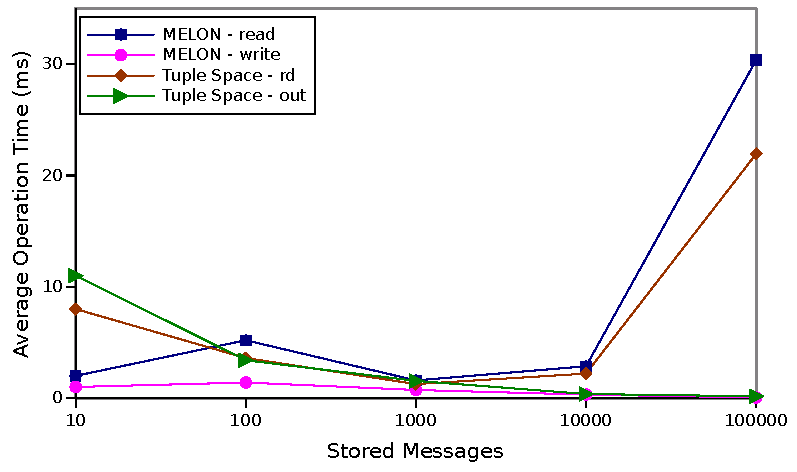
\includegraphics[width = \linewidth, clip, trim = 0px 0px 0px 0px]{figures/read_speed.pdf}
\caption{Read Speed}
\label{fig:readspeed}
\end{subfigure}%
\begin{subfigure}{.5\textwidth}
\centering
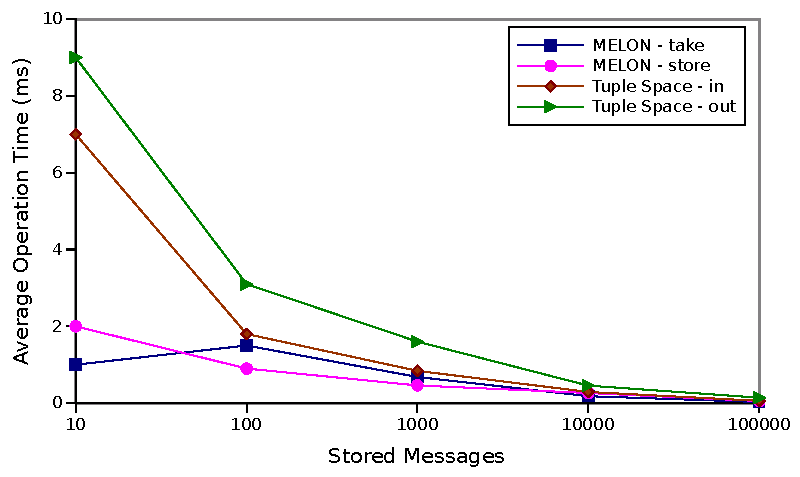
\includegraphics[width = \linewidth, clip, trim = 0px 0px 0px 0px]{figures/in_speed.pdf}
\caption{Take Speed}
\label{fig:takespeed}
\end{subfigure}

\caption{Operation Speeds}
\end{figure}

To establish a performance baseline, we measured the time for the \textbf{write}, \textbf{read}, \textbf{store}, and \textbf{take} operations directly on a local message storage and compared the results to the LighTS\cite{lights} local tuple space implementation used by LIME\cite{lime}.

%In our experiments, this cost did not become apparent until searching 100,000 messages when average time per operation increased \~9x for LighTS and \~10x for MELON, with total read time taking just under a minute. MELON is slightly slower since it must also track which messages are already read.

%When comparing \textbf{read} and \textbf{rd}, we simulate the MELON's feature of only returning unread messages by using a sequential integer ID in the tuples and performing a \textbf{rd} operation for each ID. Otherwise, LighTS would return the same tuple for each \textbf{rd} operation.  

Since LighTS and MELON search messages linearly, non-destructive reads are most affected by more stored messages. Removing messages is fast since the matching message is always the first message in the store. All \textbf{take}/\textbf{in} operations require less than 8\textit{ms} to execute on average. Storing messages is naturally faster than removing for both implementations: storing a message takes less than 10\textit{ms} on average, and usually less than 4\textit{ms}.

%MELON is slightly faster here due to differences in how removal is implemented, although average speed per operation converges as the number of operations performed increases.


%\subsection{Communication Overhead}\label{sec:overhead}

%\begin{figure}
%\centering
%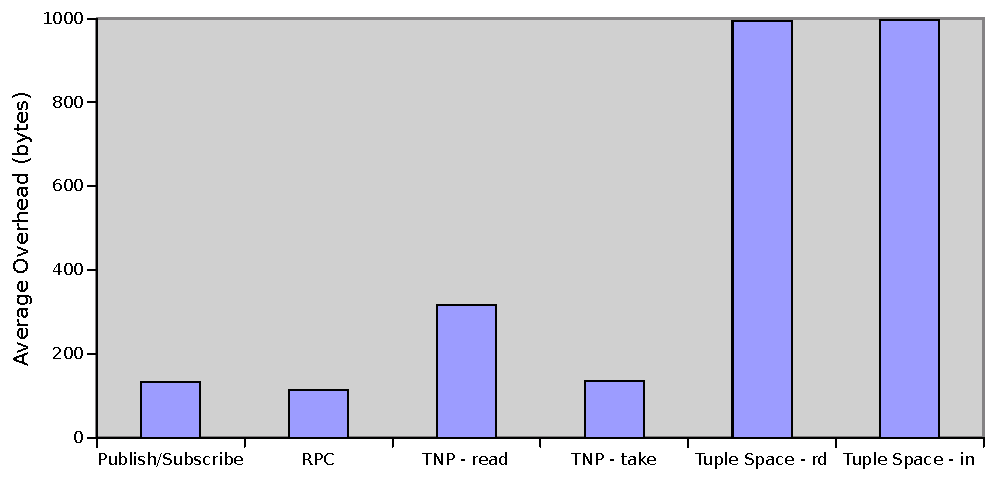
\includegraphics[scale = .34, clip, trim = 0px 0px 0px 0px]{figures/overhead.pdf}
%\caption{Message Overhead}
%\label{fig:overhead}
%\end{figure}

%For any communication library or framework, increased message size is an important factor in determining usefulness. We average the number of bytes actually sent over the network per message and subtract the 1KB application payload to determine overhead as shown in Figure \ref{fig:overhead}.

%Publish/subscribe and RPC have very low overhead and provide a good baseline. In the case of publish/subscribe, the only added information to a publication is a topic. For RPC, there is one initial exchange to find the remote object, then later messages only need the object and method names plus the payload.

%We again use the LighTS tuple space implementation to determine overhead. The serialized versions of tuples and tuple templates are very large and must be sent for each request. If simpler data structures were used, overhead would be expected to be similar to MELON's overhead for \textbf{take}.

%For MELON, \textbf{take} and \textbf{read} requests must send a message template, so the size of the request is dependent on how many values the template contains. For \textbf{read} operations, each request must also send information on previously read messages, which increases as the number of read messages increases.

\subsubsection{Message Latency}

Figure \ref{fig:latency} shows the average latency between request and receipt of a message. A single host writes out 1,000 messages with a 1KB payload, and the other hosts read the messages concurrently. Tuple spaces and MELON use the \textbf{rd}/\textbf{read} operations to retrieve the messages singularly. For publish/subscribe, latency was measured as the time elapsed between receiving sequential publications.

In these experiments, MELON and tuple spaces were the most affected by the increase in node speed and packet loss, as well as having the highest latency when nodes were at rest. MELON latency increased 29\% and tuple spaces increased 24\%. In contrast, RPC only increased 7\% and publish/subscribe actually had the lowest latency at the highest node speed. Since publish/subscribe is push-based and has very low overhead, it is able to take advantage of the increased opportunities for transferring data. On the other hand, MELON and tuple spaces have high overhead and must repeatedly request messages from remote nodes.

\begin{figure}
\centering

\begin{subfigure}{.41\textwidth}
\centering
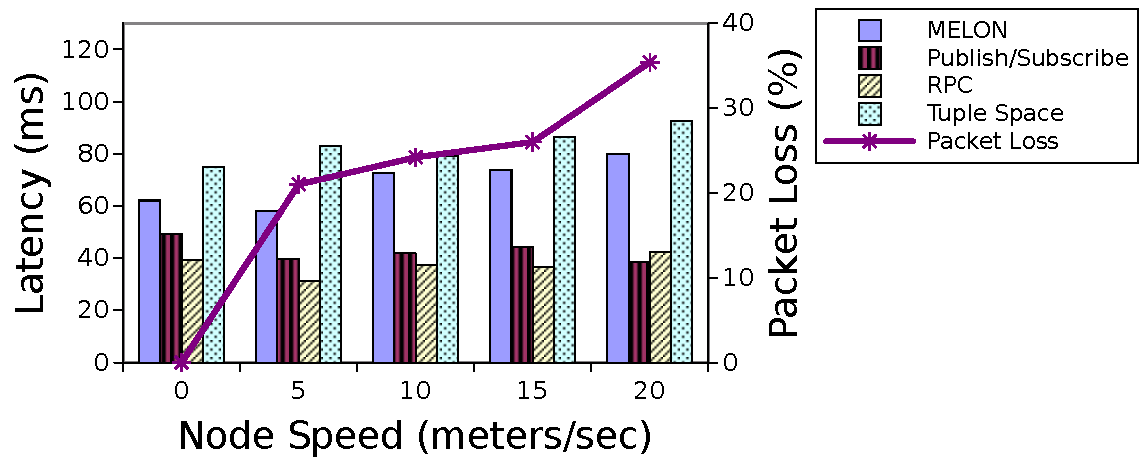
\includegraphics[width = \linewidth, clip, trim = 0px 0px 160px 0px]{figures/latency.pdf}
\caption{Message Latency}
\label{fig:latency}
\end{subfigure}%
\begin{subfigure}{.18\textwidth}
\centering
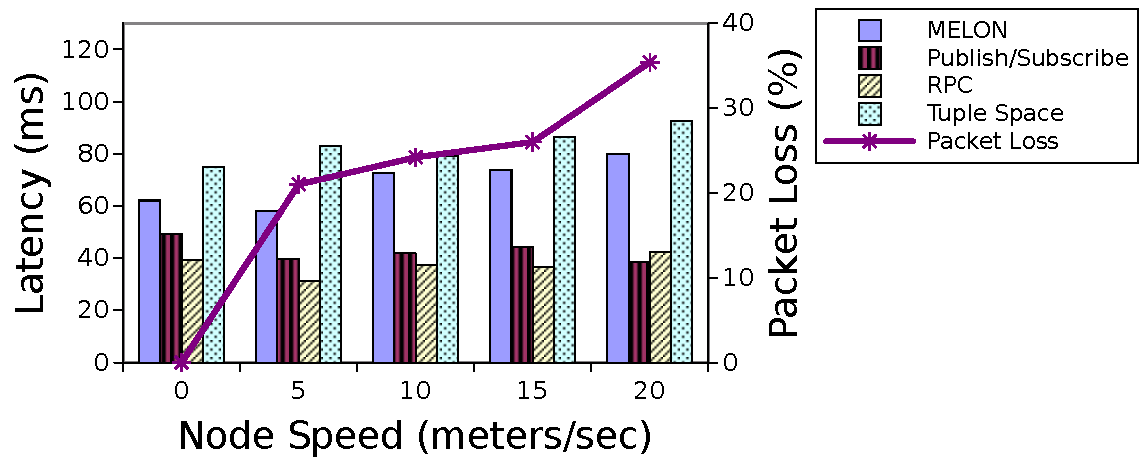
\includegraphics[width = \linewidth, clip, trim = 390px 0px 0px 0px]{figures/latency.pdf}
\end{subfigure}%
\begin{subfigure}{.41\textwidth}
\centering
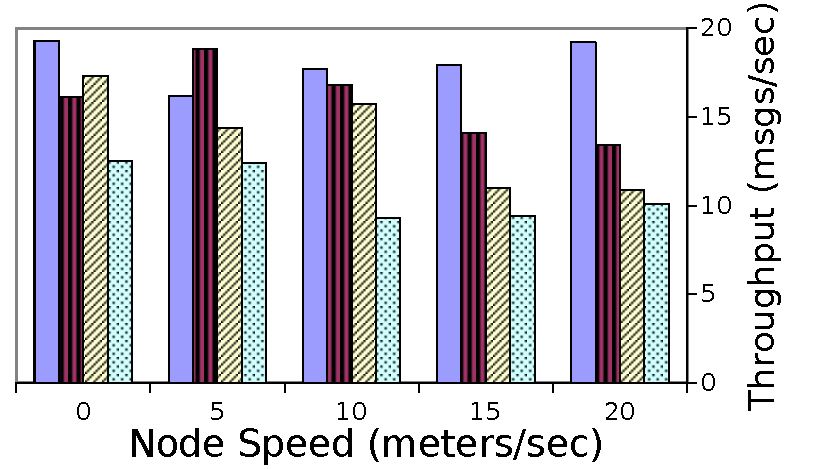
\includegraphics[width = \linewidth, clip, trim = 0px 0px 0px 0px]{figures/throughput.pdf}
\caption{Message Throughput}
\label{fig:throughput}
\end{subfigure}
\caption{Communication Performance}
\end{figure}

\subsubsection{Message Throughput}

Throughput was measured on the receiver side in messages delivered per second. Figure \ref{fig:throughput} shows the average throughput with varying node speeds. Tuple spaces perform the worst, delivering 12.5 to 10.1 messages per second. MELON provides the best performance with 19.2 to 16.2 messages per second. Publish/subscribe performs well at moderate speeds (18.8 msgs/s at 5 m/s), but packet loss reduces the number of delivered messages and throughput drops 29\% to 13.4 msgs/s at 20 m/s.

%Both tuple spaces and MELON actually improve slightly as node speed increases from 5 to 20 meters per second. Although higher node speed causes more disconnections, it also increases the likelihood nodes will be near each other during the experiment.

%\section{Related Work}\label{sec:relatedwork}

%MELON is most closely related to tuple spaces as introduced by the Linda\cite{linda} language and explored as a mobile platform in L2imbo\cite{limbo} and LIME.\cite{limerevisted} presents difficulties of implementing tuple space semantics in MANETs, including situations leading to livelocks. Other MANET tuple space adaptations include LIME II\cite{lime2}, CoreLIME\cite{corelime}, and JION\cite{join}.

%We also compare MANET performance of traditional paradigms in \cite{collins2010quantitative}. Further surveys of middleware, languages, and communication paradigms for MANET development can be found in \cite{mine} and \cite{mwtrends}.


\section{Conclusion}\label{sec:conclusion}

MELON is a new communication paradigm designed for MANET application and middleware development. It provides a unique combination of new features for interacting with a distributed shared message store, including separation of read-only messages and removable messages, private messages, bulk message operations, and tracking of read messages. In this paper we used real applications to compare MELON performance to existing communication paradigms and demonstrated acceptable performance in a MANET context.

%There are several aspects of MELON which can be explored in future work including message replication, garbage collection, and secure communication. Message replication is very useful in MANETs to overcome network partitioning and increase availability. On the other side, garbage collection of old (and replicated) messages is necessary to keep the MELON storage requirements low for small devices. While MELON does offer direct communication, encrypting private communications is necessary for full security against eavesdropping.

\bibliographystyle{unsrt}
\bibliography{refs}

\end{document}
